
\section{Abstract}
The purpose of this work is to study the feasibility of digital breast tomosynthesis (DBT) with reduced breast compression. The actual compression method will be investigated using a biomechanical breast model. The compression methodology is reproduced by means of finite element theory in order to estimate the impact of the non-uniform breast thickness on the image quality and the average glandular dose. First, the breast 3D biomechanical model is the subject of a hyper-elastic transient simulation within the ANSYS software. Second the compressed model is imported in CatSim simulation framework for X-ray computed tomography, and synthetic images are generated. Finally, the correlation between the phantom thickness and image parameters is analyzed. The biomechanical breast model will be also used to estimate the perceived pain in terms of tissues internal strain due to compression.
 Based on the analysis results, alternative compression methods will be investigated in order to improve the patient comfort and cheep a good lesion detectability and a low average glandular dose.

In this scope a biomechanical breast model has first been developed and is currently validated based on MR images of 3 volunteers. The proposed model takes into account breast heterogeneity, hyper-elasticity and patient specific geometry and tissues elasticity. Four types of tissues are highlighted: muscle, adipose tissue, glandular tissue and skin. All breast tissues are modelled as neo-Hookean materials. A particular attention is granted to modelling the breast support matrix computed of the fascia membrane. A physical correct modelling of the breast requires the knowledge of the stress-free breast configuration. Here, this reference shape (i.e. without any internal stress) is computed using an adapted prediction-correction iterative algorithm. 


\section{Introduction}
Mammography is a specific type of breast imaging that uses low-dose X-rays to detect cancer in early stage. During the exam, the breast is compressed between two plates until a nearly uniform breast thickness is obtained. This technique optimizes image quality, hence the tissue visualization and reduces the absorbed dose of ionizing photons.  But breast compression is also often a source of discomfort and sometime pain for the patient during and after the exam. Though the mammography is the most effective breast cancer screening method, the discomfort perceived during the exam could deter women from getting the test. Therefore, alternative techniques allowing reduced breast compression is of potential interest.

The aim of this work is to develop a 3D biomechanical Finite Element (FE) breast model in order to analyze various breast compression strategies and their impact on image quality and radiation dose. CatSim environment is used to create artificial breast images from numerical phantoms and to compute the corresponding averaged glandular dose. The biomechanical model estimates the compressed phantom geometry relative to the applied forces before being introduced in the image simulation workflow. From the finite element solution, the 3D strain cartography is computed as a first guess of pain and discomfort.
\subsection{Finite element breast models}
Biomechanical modelling of breast tissues is widely used in various medical applications such as surgical procedure training, pre-operative planning, diagnosis and clinical biopsy, image guided surgery and image registration, material parameter estimation. For the last 20 years several research groups have presented their breast models based on finite elements theory. One of the first breast biomechanical models based on the finite element theory is the one proposed by \cite{azar_methods_2002}. The model is used as a novel method for guiding clinical breast biopsy. The breast tissue is considered homogeneous, isotropic, incompressible and modeled as a non-linear material. The compression is modelled using virtual compression plates by applying displacements to the surface nodes. Large deformation is approximated by a sum of small increments using small-strain considerations.

Later more complex models where developed implying different types of tissues, anisotropies, large deformation theory and more complex boundary conditions. \cite{rajagopal_development_2004} developed a model based on large deformation mechanics in order to validate the assumption of isotropy, homogeneity and incompressibility of soft tissues. The material models where computed using the bibliography data only. The method was validated experimentally using silicone gel phantoms subject to gravitational loading. \cite{rajagopal_modelling_2007} also studied the effect of modelling the breast skin layer. And as \cite{pathmanathan_predicting_2008} research team they found that modelling the skin results in an underestimation of breast displacements. 

\cite{han_development_2012} developed a bio-mechanical breast model for surgical simulations. In their model 3 types of tissues are considered: muscle, glandular and adipose tissues. \cite{gamage_modelling_2012} introduced the pectoral muscle in the breast mechanical model and showed that the muscle should be accounted in the modelling.

 The anisotropic effect of Cooper's ligaments was introduced for the first time by \cite{pathmanathan_predicting_2008} and took up again by \cite{han_development_2012}. Both teams have introduced an additional factor in the stress-strain energy function describing the transverse isotropic properties. They also	 considered the breast heterogeneity by modelling adipose tissue and fibro-glandular tissues with different materials. However, the model was not validated using clinical data. A new modelling method for Cooper's ligaments vas proposed by \cite{georgii_simulation_2016}. They added a generic ligaments model based on a mass-spring system to the finite element model. 
 
 The deformation of an elastic body is typically performed by specifying appropriate boundary conditions. Almost all biomechanical breast models are based on fixed boundary conditions, i.e. the nodes lying on the posterior face of the breast are defined with zero-displacement proprieties.
\cite{payan_application_2012} replaced the "fixed" boundary conditions by a "sliding" region between the posterior part of the breast and anterior part of the pectoral muscle. Recently the \cite{patz_sliding_2015} team have presented a new time-preserving method to model the sliding motion. The sliding method is based on fixed boundary conditions in conjunction with an explicit update computed using the resulting internal forces of the elastic material.

The bibliography presents 3 main limitations for breast mechanical simulation:
\begin{enumerate}
\item Unknown stress-free breast configuration. Since, for all in-vivo studies, breast geometry is extracted from the MRI data, the measured configuration represents the breast subject to gravity loading. Thus, for a Finite Element modeling it is very important to accurately estimate the unloaded (i.e. stress-free) configuration.
\item Unknown elastic parameters of breast soft tissues. The bibliography shows a very large interval of elastic parameters depending of the experimental methods and made assumptions.
 \item Breast tissues are known to be extremely soft. Very large deformation of materials implies excessive elements distortion. A poor mesh quality can lead to inaccurate results and numerical instability.
\end{enumerate} 

\subsection{Breast tissue biomecanical modeling}
Global breast mechanics are governed by breast tissue compositions and their individual mechanical properties. Therefore, an accurate breast model stands on a good knowledge of breast anatomy and on full characterization of the mechanical behavior of the involved tissues.

 Multiple studies have show that female breast composition and so its mechanical behavior undergo substantial changes during the lifetime.
The first studies on estimation of mechanical proprieties of breast tissues were done in diagnostic purposes. Presence of tissues with mechanical proprieties different from the breast-like tissues implies breast anomalies. The study published by \cite{krouskop_elastic_1998} show the difference in stiffness between breast tissues and carcinomas. In this study authors supposed that the difference in breast global stiffness is only due to the changes in breast tissues compositions and not in changes of the individual material property. Therefore, they have studied ex-vivo 142 tissues samples from different subjects and they assumed their homogeneity. The samples were representing 4 type of tissues: adipose tissue, glandular tissue, fibrous tissue and carcinoma. They showed that due to the difference in material stiffness measured using elastography they are able to detect pathological changes in breast tissues and moreover they can estimate elastic parameters of normal tissues images from elastography.  

%Later  

 Later, several research groups have presented values of elastic modulus of adipose and glandular tissues. The range of elastic parameters is going from 0.1 kPa to 271.8 kPa (see table \ref{elastic_modulus_table}). Such big variation can be explained by the differences in the used methods but also by the different physical condition, age or period of the menstrual cycle of the participants. \cite{lorenzen_menstrual-cycle_2003} found that during the menstrual cycle, due to the hormonal changes, the elastic properties of the glandular tissues can change by about 30 \%. 
%\begin{table}[h]
\begin{sidewaystable}
    \centering
   \begin{tabular}{c|c|c|c|c}
   \hline
  \multicolumn{5}{c}{\textbf{Ex-vivo estimation}}\\
   \hline
    Author & Method & Material model&\multicolumn{2}{c}{Material constants} \\
    \cline{4-5}
    &&& Adipose & Glandular\\
    \hline
    \cite{krouskop_elastic_1998} - 5\% precomp. & identation & Linear elastic & E=20 kPa & E=33 kPa \\
    \cite{krouskop_elastic_1998} - 20\% precomp. & identation & Linear elastic & E=20 kPa & E=57 kPa \\
    \cite{wellman_breast_1999}- 5\% precomp. & identation & Linear elastic & E=6.6 kPa & E=33 kPa \\
    \cite{wellman_breast_1999}- 15\% precomp. & identation & Linear elastic & E=17.4 kPa & E=271.8 kPa \\
     \cite{samani_elastic_2007} & identation & Linear elastic & E=3.25 kPa & E=3.24 kPa \\
   \hline
  \multicolumn{5}{c}{\textbf{In-vivo estimation}}\\
   \hline
     \cite{van_houten_initial_2003} & MRE & Linear elastic & E=17-26 kPa & E=26-30 kPa \\
     \cite{carter_determining_2009} & MRI & Neo-Hookean & $C_{10}$=0.2-1 kPa & $C_{10}$=0.4-0.8 kPa \\
     \cite{han_development_2012} & MRI & Neo-Hookean & E=1 kPa & E=0.22-43.64 kPa \\
     \cite{gamage_modelling_2012} & MRI & Neo-Hookean & $C_{10}$=0.1 kPa & $C_{10}$=0.1 kPa \\
     \cite{Rajagopal_creating_2008} & MRI & Neo-Hookean & $C_{10}$=0.08 kPa & $C_{10}$=0.13 kPa \\
    
    
    \end{tabular}
     \caption{Elastic modulus of adipose and glandular tissues}
     \label{elastic_modulus_table}
\end{sidewaystable}
%\end{table}

An important difference in the estimated elastic modulus of soft tissues is observed between the linear elastic and hyperelastic models. In the l studies where authors are using a hyperelastic Neo-Hookean models with in-vivo measurements, the range of the adipose and glandular elastic modulus is lower than 1kPa, compared to an average of 20-30 kPa given be the linear models with ex-vivo measurements. 

\cite{carter_determining_2009} used a Finite Element breast model considering 3 types of tissues: adipose tissue, glandular tissue and skin. All 3 tissues were modelled as Heo-Hookean incompressible materials. Since the soft tissues are of the same density as the water, the submerged in water breast was considered to have zero internal stress.  The elastic parameters are estimated by minimizing the difference between computed and measured prone breast configurations. For this model the authors obtained elastic modulus equal to 0.2 kPa for adipose tissue, 0.4 kPa for glandular tissue and 10 kPa for skin.

 \cite{gamage_modelling_2012} have considered the breast as a homogeneous material but have also included the pectoral muscle in the biomechanical model. Both tissues were modelled as hyperelastic materials. They obtained 0.1 kPa for elastic modulus of the homogeneous breast and 0.52 kPa for muscle. 
  
 \cite{van_houten_initial_2003} have considered also the Poisson Ratio as a variable. The estimation is done in in-vivo conditions (based in magnetic resonance elastography). The authors assume linear material behavior therefore the elastic modulus and Poisson Ratio are computed from the 2 Lam\'e modulus. They found that the Poisson Ratio for adipose tissue lies between 0.34-0.4 and for glandular tissue around 0.4.

Previously listed researches clearly showed the variability of elastic modulus of the same tissue between and within individuals. \cite{eder_comparison_2014} made a large analysis of all existing material models. According to their findings many of proposed in the literature parameters are too stiff, and namely those that are obtained by indentation ex-vivo test. The more reliable values are given by \cite{Rajagopal_creating_2008}, the other values permitting not enough deformation due to the gravity loading.
\subsection{Skin biomechanical modeling}
The skin mechanical parameters are also important in breast mechanics. Only \cite{carter_determining_2009} have included the skin in the identification process of the breast soft tissues elastic modulus. The authors modeled the skin as a Neo-Hookean incompressible material, and they obtained an elastic modulus equal to $10kPa$. 

\cite{sutradhar_vivo_2013} published a complete study of breast skin estimating the thickness and elasticity for 16 different breast regions. The study was done on 23 female volunteers aging from 29 to 75 ears. With in-vivo suction experiments they found an average thickness of $1.55mm$ and an elastic modulus of 334kPa. They also showed the regional variation of skin thickness: according to the authors the lateral region thickness is the thinnest among all the breast regions followed by superior/inferior part (without any significant differences) and the medial region. Concerning the radial distribution, the interior region closer to the nipple was more thin than the exterior radial part of the breast. A similar regional variation study was done on the skin elasticity. It was found no significant variation of elastic modulus in radial direction. The modulus was found grater in the superior and lateral part than in the inferior and medial parts respectively. An additional measurement was done in order to compare the skin elastic modulus in supine and upright position with no significant differences found.

 Other research on skin elasticity are available, but they are not specific to the breast skin. \cite{hendriks_relative_2006} estimated in-vivo skin proprieties by suction testing. The skin was considered as a homogeneous, isotropic, incompressible, hyperelastic material. The study was performed on 14 subjects and the obtained average of elastic modulus for skin was $58,4 kPa$.  

\subsection{Stress-free breast configuration}
As mentioned before, in the breast configuration given by MR images the soft tissues are pre-stressed due to in-vivo conditions (i.e gravitational forces). In order to apply the continuum mechanics theory, an initial stress-free breast shape is needed. 

One of the existing methods for estimating such a stress-free shape is the backward finite element formulation used by \cite{pathmanathan_predicting_2006} in his biomechanical model. The method is based in the reformulation of the virtual work equation, where the residual forces are expressed in terms of unknown reference state coordinates. 

\cite{carter_biomechanical_2009} addressed the same problem solving an iterative sequence of forward deformations where the only unknown is the reference configuration. First, the reference configuration is assumed to be equal to the prone breast configuration. Second the gravity loading is applied in order to compute a first estimation of the prone configuration. From the first estimation of deformed state a difference in node location is computed. Then, the reference state is perturbed accordingly to the computed difference until convergence is achieved.

 Later \cite{eiben_breast_2014} refined the method by translating the difference location vector from the deformed space to the reference space by multiplying the vector with the inverse deformation gradient.   \cite{eiben_breast_2014} compared the two previous methods; according to the authors the backward formulation methods exhibits excellent results only when elastic parameters are well known. Since in the prone-supine breast deformation context the elastic parameters are unknown, there is no significant numerical difference between the two methods.   
 
  This problem was raised for the first time by \cite{kuhlmann_mechanical_2013}. To solve the large deformation problem, they proposed a coupled Eulerian-Lagrangian FE method. According to the authors this method is more relevant for breast soft tissues but is highly time-consuming.   
 

\section{Materials and methods}
\subsection{Breast Anatomy}

A good knowledge of anatomical breast structure and its composition is necessary when one is developing a biomechanical model.  The tissues distributions and their biomechanical properties define the global breast mechanics. 

 \subsubsection*{Breast embryogenesis}
The breast gland have the same ectodermal origin  as skin glands.

\begin{center}
\begin{figure}[!htb]
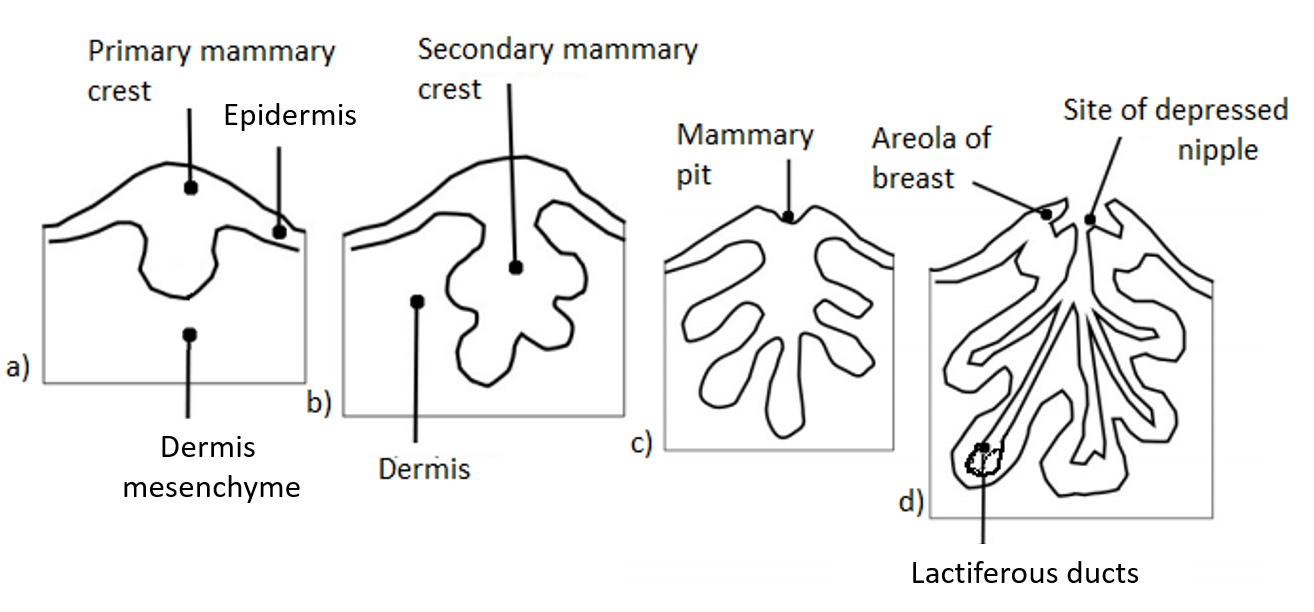
\includegraphics[width=\textwidth,height=\textheight,keepaspectratio]{figures/breast_evolution_my.png} 
\caption[Breast embryogenesism: stages of formation of the duct system. the ectoderm is responsible for duct system and alveoli, the mesenchyme is responsible for the connective tissue and vessels] {Breast embryogenesism: stages of formation pf the duct system. the ectoderm is responsible for duct system and alveoli, the mesenchyme is responsible for the connective tissue and vessels  ~~ ~\cite{shiffman_melvin_a_breast_2008}. }
\label{breastembryogenesis}
\end{figure}
\end{center}

 During the first trimester of intrauterine growth,  the mammary crest develops in the embryo ectoderm (fig \ref{breastembryogenesis}.a), 16-24 solid cords of epithelial cells are growing down into the dermis (fig. \ref{breastembryogenesis}.b). Later, these cords will evolve in the lactiferous ducts and alveoli (fig. \ref{breastembryogenesis}.d). At the full-term fetus there is already a simple network of branching ducts. The glandular elements, generally do not appear until adolescence. In the adolescence, under hormonal simulation, the breast buds enlarge on the chest wall and eventually on the axilla region , becoming palpable discs beneath the nipple. The ducts grow into the soft tissues and the lobular differentiation begins \cite{kopans_daniel_b_breast_2007}. 

\begin{center}
\begin{figure}[!h]
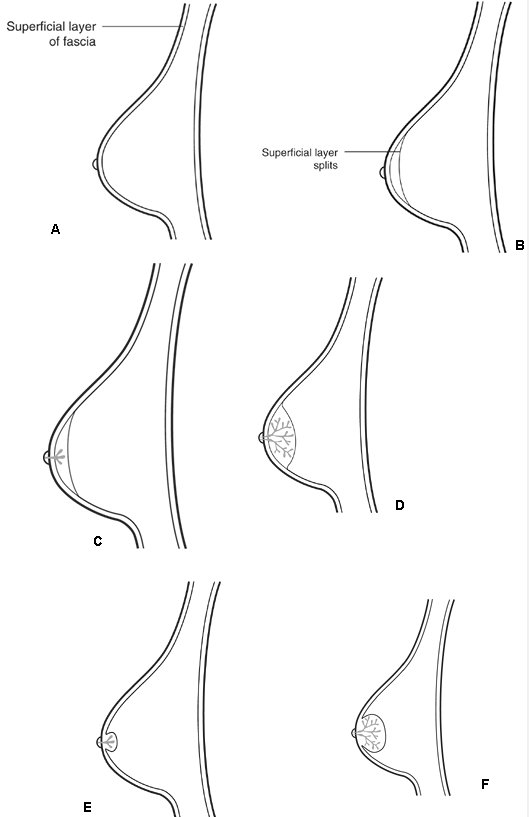
\includegraphics[height=0.7\textheight,keepaspectratio]{figures/breastEvol_fascia.png} 
\caption[Breast development sequence in the subcutaneous tissues. A-D Mammary bud development by spleeting the superficial fascia in 2 layers. E-F Mammary bud development]{Breast development sequence in the subcutaneous tissues. A-D Mammary bud development by sleeting the superficial fascia in 2 layers. E-F Mammary bud development, reproduced from  ~~\cite{kopans_daniel_b_breast_2007}  }
\label{breastevol_fascia}
\end{figure}
\end{center}

\cite{kopans_daniel_b_breast_2007} analyzed breast development sequence in the subcutaneous tissues. According to the author the evolution of breast within the fascial system is unclear, two possible evolution are presented: 
\begin{enumerate}
\item The superficial fascia split in two layers forming the deep and the superficial fascia layers. With the breast forming in between (fig.\ref{breastevol_fascia}.A-D).
\item The elongating ducts invaginate the fascia which end up 
enveloping the gland (fig.\ref{breastevol_fascia}E-F)
\end{enumerate}


\subsubsection*{External structure}
The breast is an apocrine, tear-shaped gland \cite{valerie_mammographic_2011}. Anatomically, the adult breast sits atop the ribcage, between the clavicle and the sixth to eighth ribs. The breast tissue extends horizontally (side-to-side) from the lateral sternal line out to the midaxillary line (see fig.\ref{fig:breast_quadrants}).

The adult breast size variates within intra and inter individuals. The asymmetric breast within individuals is relatively usual. Therefore some research groups have defined geometry metrics in order to characterize the variation of breast size  and its asymmetry. By definition the base of the breast is the portion adjacent to the chest wall, the apex is the nipple-areola complex (fig. \ref{fig:breast_apex}), the breast projection is the distance from the apex to the breast base. 


\begin{figure}[h]
\minipage{0.1\textwidth}
\endminipage\hfill
\minipage{0.5\textwidth}
  
\includegraphics[width=\linewidth]{figures/breastBase.PNG}
  \caption{Base and apex of the breast}\label{fig:breast_apex}
\endminipage\hfill
\minipage{0.2\textwidth}
  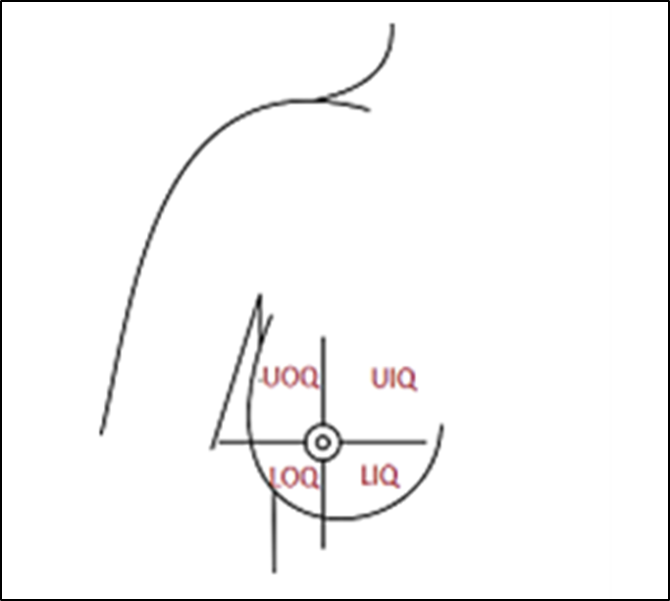
\includegraphics[width=\linewidth]{figures/Breast_quadrants.png}
  \caption{Four breast quadrats}\label{fig:breast_quadrants}
\endminipage\hfill
\minipage{0.1\textwidth}
\endminipage\hfill
\end{figure}
In medical imaging, to describe location in the breast, four quadrants are defined: upper outer quadrant (UOQ), upper inner quadrant (UIQ), lower outer quadrant (LOQ), lower inner quadrant (LIQ)(see fig.\ref{fig:breast_quadrants}).   The natural landmarks of thorax surface are the nipple, the inframammary fold, the jugular notch, clavicle, sternal angle and the axilla. Some of these structures are used to describe locations of normal anatomy and pathology.

\begin{center}
\begin{figure}[!h]
\centerline{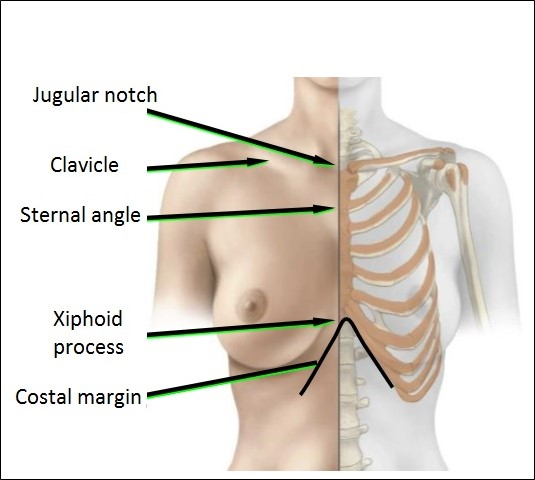
\includegraphics[width=0.5\textwidth,height=0.5\textheight,keepaspectratio]{figures/surfacelandmarks.jpg} }
\caption{Thorax surface landmarks.}
\label{thorax}
\end{figure}
\end{center}

Studies on the breast dimensions have been done essential for cosmetic and reconstructive surgery. \cite{catanuto_experimental_2008} presented several parameters which can characterize unambiguously the breast shape, among them the curvature of the thoracic surface has been identified as the most relevant. The superior half of the healthy breast was shown to be
almost flat especially in the inner quadrants (fig. \ref{fig:breast_quadrants}) while moving towards the upper outer quadrants curvature becomes negative. According to the authors, the breast deformation can not be described by volume measurements only.

The skin is the covering breast layer which provides protection and receives sensory stimuli from the external environment. It is a heterogeneous organ composed of 3 layers, see fig. \ref{skinanatomy} (\cite{gefen_mechanics_2007}): 
\begin{enumerate}
\item epidermis (dead cells) mainly composed of keratin, it's thickness ranges between 50 and 100 $\mu$m ;
\item dermis: composed of collagen and elastin fibers in a viscous matrix made of water and glycoproteins, with a thickness between 1-3 $mm$;
\item hypodermis, mainly composed of adipocytes cells, it's thickness variate depending on the individual and location area between 1 and 7 $mm$.
\end{enumerate}


\begin{center}
\begin{figure}[!h]
\centerline{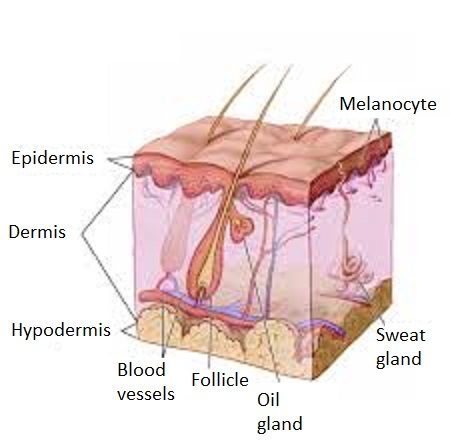
\includegraphics[width=0.5\textwidth,height=0.5\textheight,keepaspectratio]{figures/skin.jpg} }
\caption{Skin anatomy}
\label{skinanatomy}
\end{figure}
\end{center}


The breast skin is thickest at the base of the breast ($\sim$ 2 $mm$), and becomes thinner approaching to the nipple ($\sim$ 0.5 $mm$) (fig. \ref{breastanatomy}). At the nipple areola region, the skin thickness measure 4-5 $mm$ (\cite{valerie_mammographic_2011}). \cite{ulger_harun_effect_2003}
described the range of normal breast thickness using a film-screen mammographic technique. According to the authors the breast skin ranges between 0.50 mm and 3.10 mm, with significant differences between the 4 regions in the same breast. They also found that, even if the breast size increases with age, the skin thickness decreases in all regions.

\subsubsection*{Internal structure}

Breast heterogeneous structure includes a mixture of parenchyma and adipose tissue (see fig. \ref{breastanatomy}). The breast parenchyma consists of: glandular components, lymphatic network and blood vessels (\cite{clemente_anatomy:_2011}). Cooper's ligaments and fascias are the supporting system of the breast, their interconnection and intersections with the pectoral muscle fix and support the breast soft tissues.

 A layer of adipose tissue and connective fascia separates the breast from the pectoral muscle forming a retro-mammary fat space. Adipose tissue is also the predominant tissue of the breast that fills up depressions between the two layers of fascia. In the intra-fascial space, fatty tissue surrounds and is dispersed among the glandular structures \cite{valerie_mammographic_2011}. Fat properties and its spatial distribution gives the breast a soft consistency. The amount of fat determines the size of the breast. The aim of this tissue is to protect the lobes and the lactiferous ducts.

Glandular tissue is represented by breast lobes. A healthy female breast is made up of 12-20 lobes. They are distributed centrally and laterally within the breast. The total amount of glandular tissue depends on the hormonal fluctuation, age and physical state.  Mammary ducts arise from the lobes as branches and connect them to the female nipple. There are about 10 duct system with a tree-like structure in each breast that carry the milk from the lobes to the nipple. The dark area of skin surrounding the nipple is called the areola. \cite{huang_shih-ying_characterization_2011} have studied the breast shape and fibro-glandular distribution using dedicated breast CT images. This study shows that the glandular tissues is situated in the central portion of the breast. In prone position about 60 $\%$ of glandular tissues is located near to the nipple. A mean percentage of glandular tissue was computed by \cite{yaffe_myth_2009}, the values varied from 13.7$\%$ to 25.6 $\%$ within different groups. They also mentioned a drop in glandular fraction with the advancing age. 


\begin{center}
\begin{figure}[h]
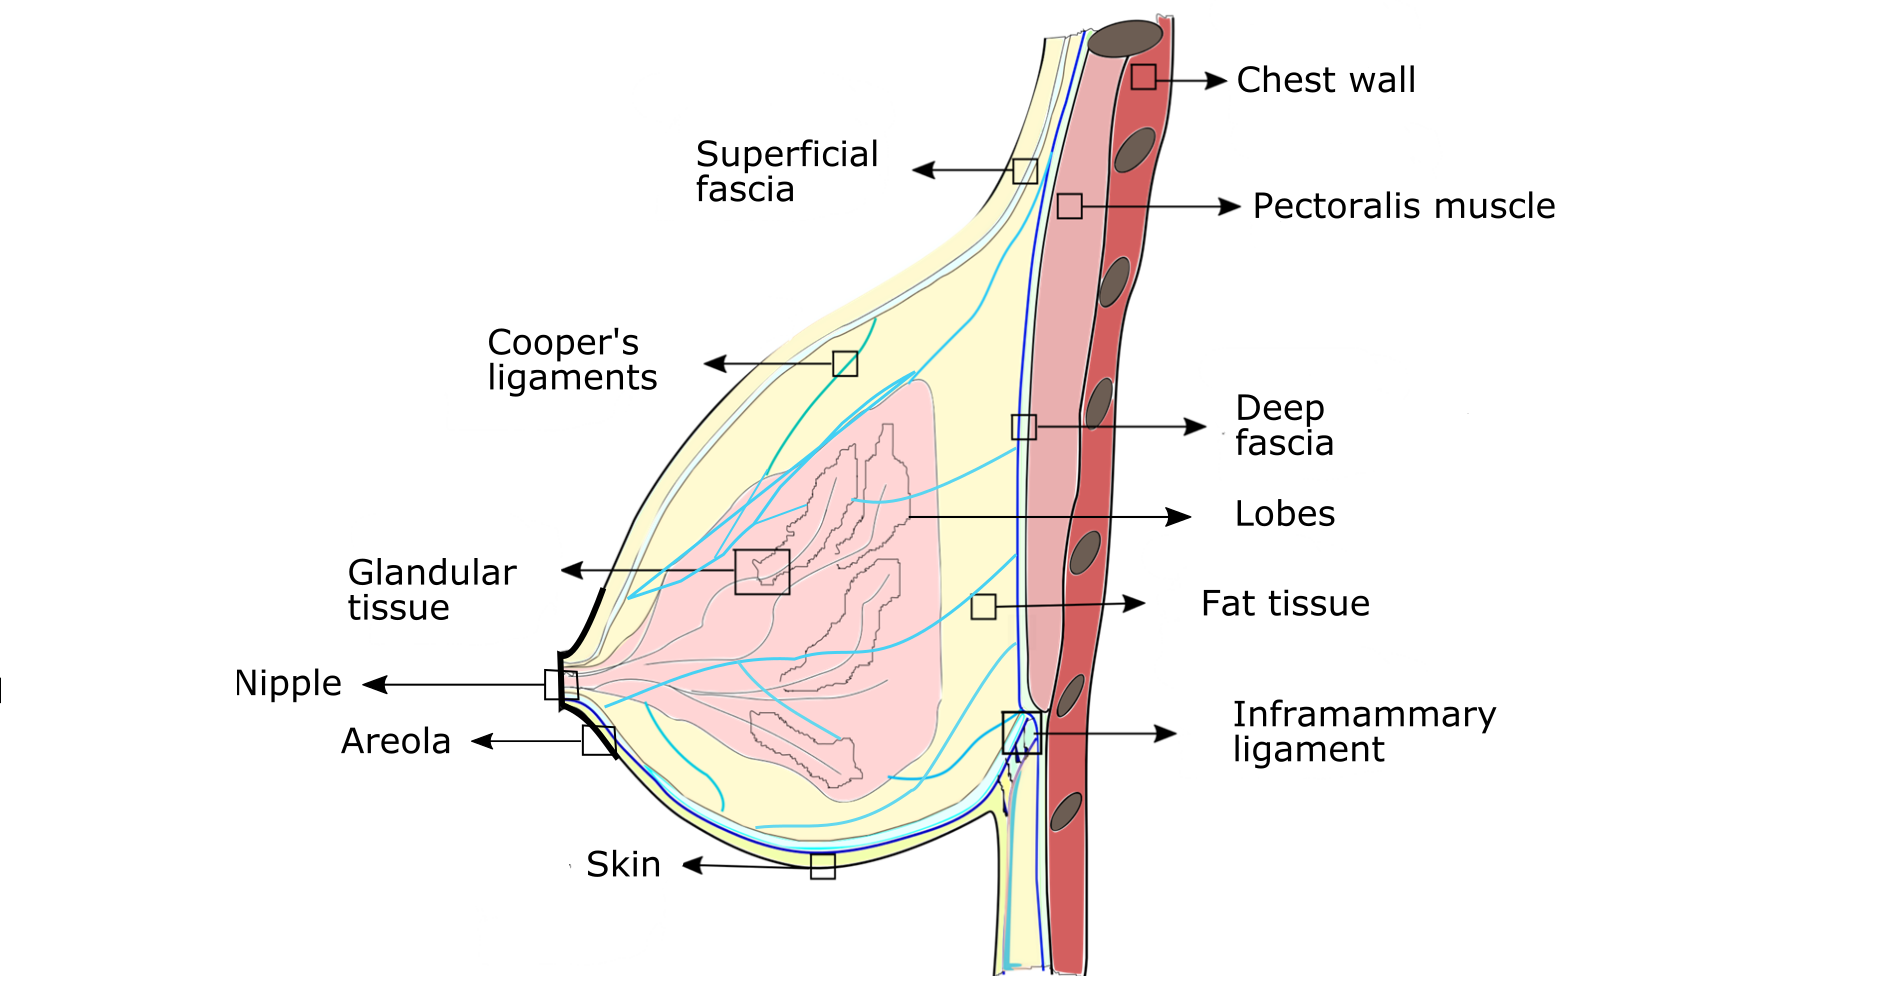
\includegraphics[width=\textwidth,height=\textheight,keepaspectratio]{figures/anatomieSeinEuBlack.png} 
\caption{Breast anatomy}
\label{breastanatomy}
\end{figure}
\end{center}

Connective tissue is represented by Cooper's ligaments and fascial system.  Cooper's ligaments are fibrous membranes that incompletely sheathe, but support the breast lobes. Fascia mammae is also a fibrous membrane divided into a superficial and a deep layer which completely envelope the breast. Cooper's ligaments run from the superficial fascia through the breast and attach to deep fascia (see Fig. \ref{breastanatomy}). The intersection of the two fascias in the region of the 5th and 6th rib forms the inframammary crease ligament. These ligaments extend all around the breast to form a stiff 3D structure fixing the breast tissues to the chest wall. The connective tissue provides support to the breast and gives its shape. This fibrous structures are not elastic as breast soft tissues. They will maintain their deformed state after a stretching which occurs within an increase in breast volume. For example, the pendulous breast appearance after the pregnancy or a weight gain followed by a loss of weight is known as "Cooper's droop" phenomenon.  \\

The lymphatic and venous drainages of the breast are of great importance in the spread of carcinoma. When a female is developing a breast cancer, usually the primary tumor is developed in the epithelial cells. Then malignant cancer cells spread by entering lymphatic capillaries and proceed to lymph nodes, where they may multiply to form metastatic secondary tumors. Spread of tumor cells also occurs by way of venous capillaries to larger veins and then to more widespread organs.

The lymphatic system is a vessel network which insures the transportation of white blood cells from tissues into the bloodstream. The majority of intramammary nodes are associated with the upper outer breast tissue and the lower outer part of the breast (more details in \cite{kopans_daniel_b_breast_2007}).  All intramammary lymph nodes are in the lateral half of the breast along the margin of the breast parenchyma.  Lymphatic drainange of breast extends from the subareolar plexus deep to and around the nipple (see fig. \ref{lyphaticDrainage} ).

The blood supply from the breast comes primarily from the internal mammary artery named successively subclavian, axillary, and brachial artery (see fig. \ref{lyphaticDrainage}), from which lateral and internal thoracic artery runs underneath the main breast tissue.

	
\begin{center}
\begin{figure}
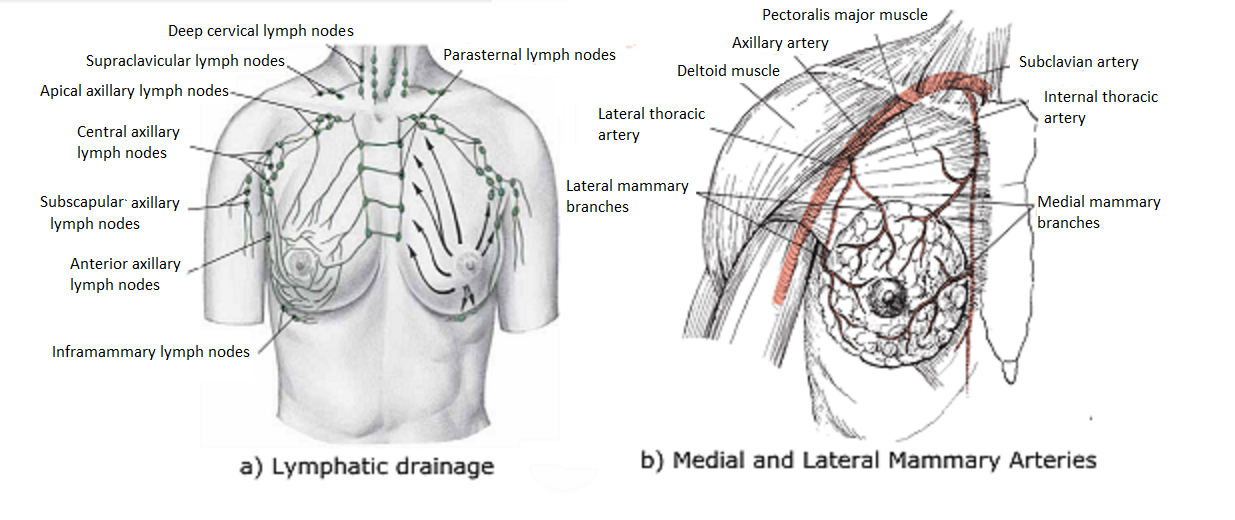
\includegraphics[width=\textwidth,height=\textheight,keepaspectratio]{figures/lyphaticDrainage.PNG} 
\caption[Lymphatic system and Mammary Arteries for adult female breast]{Lymphatic system and Mammary Arteries for adult female breast.(Reproduced from \cite{clemente_anatomy:_2011})}
\label{lyphaticDrainage}
\end{figure}
\end{center}




\subsubsection*{Breast texture changes}
The female breast undergoes substantial changes during the lifetime.  The main part of them is caused by hormones and by woman's physiological condition. Important changes in female breast stiffness and composition occur during the menstrual cycle, pregnancy and menopause. 
There are 3 important changes during the menstrual cycle caused by hormonal changes \cite{valerie_mammographic_2011}. During the first phase the estrogen (female hormones) diffusion stimulates epithelial cell multiplication and enlargement of ductal structures; next, during ovulation epithelial cell begin to grow in the lobule due to progesterone hormones, an increase in blood flow is also noticed; in the last phase, the ductal structures and lobes support an involution and regression process. It must be mentioned that not all lobules regress, therefore during a menstrual cycle new lobules can be created.  

The work by \cite{lorenzen_menstrual-cycle_2003} showed that during the premenstrual phase the stiffness of fibro-glandular tissue and glandular tissue can change by 30\% and 14 \% respectively. They also show that in the middle of the  menstrual cycle, the parenchyma volume increases of 38\% and the water content by 24.5\%. As the breast content shows a variability between and within subjects, an accurate breast biomechanical model must take into consideration the subject specific variations. 

The menopausal breast will contain a larer fraction of fatty tissues. During the first four years after menopause the breast is the subject of an atrophy process. The atrophy begins medially and posteriorly, then laterally, working its way to the nipple \cite{valerie_mammographic_2011}. In this period the breast will lose the supportive tissues by replacing it with fat. Therefore, the breasts change in shape and have a more pendulous aspect.


\subsection{Volunteers and MRI acquisition}
Breast mechanics is strongly dependent on breast anatomy and structure. A good modeling implies an accurate definition of the heterogeneous geometry and boundary conditions. In order to have a realistic estimation of in vivo conditions the entire thoracic cage is included on finite element simulation. Only the MRI images can offer all the information necessary for the construction of the finite element mesh. First, the MRI modalities permit to have a lager field of view such that the breast geometry with the thoracic cage are imaged. Secondly, during the MR image acquisition, the interactions between the breast and the scanner tube are limited, which permits to have simplified boundary conditions in comparison with others images modalities. And finally, the MRI images have a high spacial resolution in order to map accurately the different breast tissue.
     
All volunteers taking part of this study have agreed to participate in the experiment within a pilot study approved by an ethics committee. The data base contains breast images of two women within 50 years old with various breast dimensions. Three different positioning configurations are considered for each volunteer (see fig \ref{breastpositions}): prone, supine and supine titled. The positions have been chosen in order to assess the largest possible breast deformation with minimal contact area between the patient and the MRI scanner tube. We must mention that the MRI tube is very narrow, thus the possible body positions are limited, especially for the volunteer with large breast sizes.  

\begin{center}
\begin{figure}[H]
\centerline{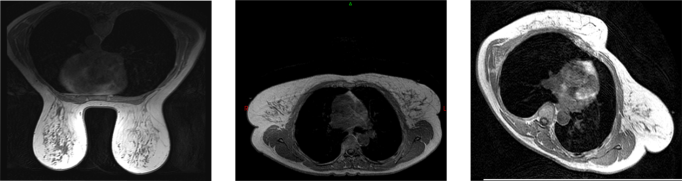
\includegraphics[width=\textwidth,height=\textheight,keepaspectratio]{figures/breastpositions.png} }
\vspace{15px}
\centerline{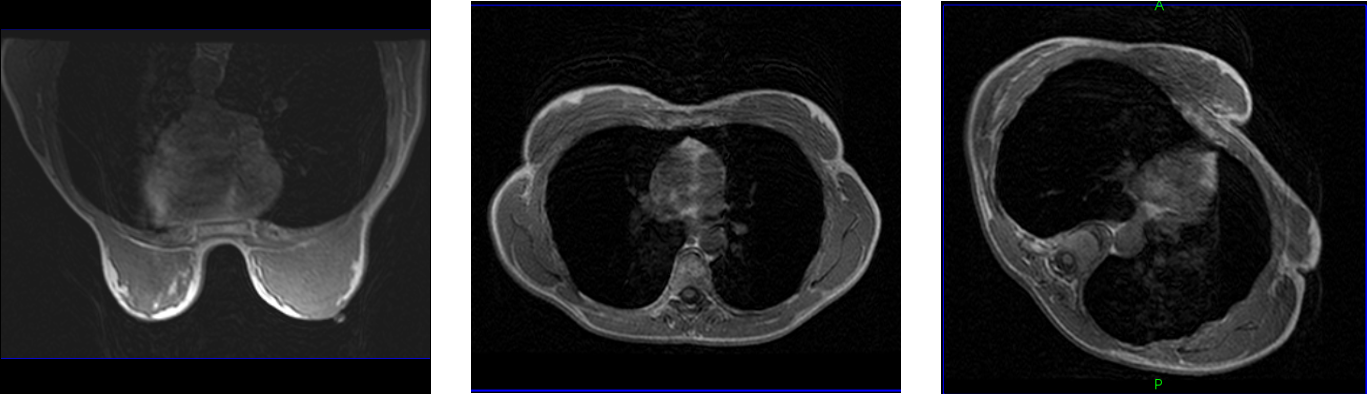
\includegraphics[width=\textwidth,height=\textheight,keepaspectratio]{figures/subject2.png} }
\caption{Three breast configuration under gravity loads: a) prone position; b) supine position c) supine tilted. Sunject 1 in first line, subject 2 in the second line.}
\label{breastpositions}
\end{figure}
\end{center}

 Before image acquisition, each volunteer was asked to fix 10 fiducials markers on her chest and the surface of the breast as shown in fig \ref{fiducial_position}. The breast tissues are known to be very soft, therefore the most part of the breast area suffer elastic deformations during the position changing. There are very small regions where the elastic deformation can by neglected as: notch-sternal angle segment, clavicle, base of the breast (under inframammary ligament) (fig. \ref{thorax}). These areas are rich in fibrous tissues which attach the skin to the thorax bone structure. In order to accurately compute the rigid body displacement during the subject re-positioning inside the MRI tube, more than 3 fiducials are needed. Considering the limited area, only 4 markers are placed on the fixed part of the chest in order to define a rigid body reference system. This set of markers will be used to compute the rigid transformation between two different body positions. The other six markers are placed to track the breast deformation and will be used to estimate the model accuracy. As the largest breast deformation is expected in the two lower breast quadrants, the markers measuring the displacement are placed respectively in this region.  
 
 
 The images were acquired with a Siemens 3T MRI scanner using T2 weighted image sequence. The image resolution in plane is of 0.5x0.5 mm and 0.6 mm slice thickness. During image acquisition, it was verified that the contact between the breast and the MRI scanner or breast and body (arms or thorax) is minimized.


\begin{center}
\begin{figure}[H]
\centerline{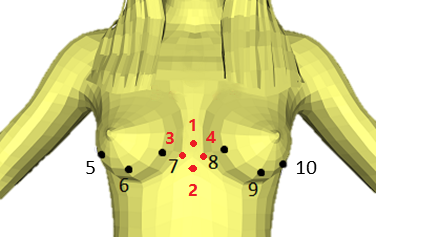
\includegraphics[scale=0.7]{figures/fiducial_position2.png} }
\caption{Graphical fiducial markers position on the woman chest.}
\label{fiducial_position}
\end{figure}
\end{center}

\subsection{Image pre-possessing}
During the imaging process the volunteers are going in and out of the MRI scanner. Therefore, the breast undergoes not only an elastic transformation but also a rigid one. Simulation of breast deformation under gravity loading assumes that the breast support (rib cage) is fixed and the breast displacement is due to gravitational forces only. In order to meet the simulation conditions, the breast rigid transformation is computed using fiducials and image registration methods. 

Next the MRI images are used to generate the patient specific finite element mesh. In this purpose the images are segmented in order to differentiate four types of tissues: glandular tissue, adipose tissue, pectoral muscle and skin.   

\subsubsection*{Image registration}
Image registration is performed considering a rigid body transformation: rotation and translation of the body inside the MRI scanner.  During the body re-positioning the breast fulfil an elastic transformation. Excluding the soft tissues from the registration process will increase considerably the results accuracy. Thus, for the rigid registration processes the image field of view is reduced to the rib cage only. 

The image registration process is performed in 2 steps:
\begin{enumerate}
\item An initial rigid transform is computed by registering the 4 points corresponding to the 4 reference markers (fiducial markers 1-4 in fig \ref{fiducial_position}). The transformation is estimated using the iterative closest point (ICP) algorithm minimizing the mean Euclidean distance between the 4 points.
\item A second optimization process is performed based on the image grey intensity using gradient descent method. At this step the metric function is computed using the normalized cross-correlation function. At the first iteration of the optimization process the transformation is initialized with the results from the initial step.

\end{enumerate}

 The final transform is applied to the whole image such that the breast will follow the movement of the rib cage.

\subsubsection*{Image segmentation}
Image segmentation was performed using the semi-automated active contour method implemented in ITK-snap software. First the breast tissues and pectoral muscle masks were computed from the whole image. Then, the breast tissues are divided in glandular and adipose tissue (see fig. \ref{femesh}). 

\begin{center}
\begin{figure}[h]
\centerline{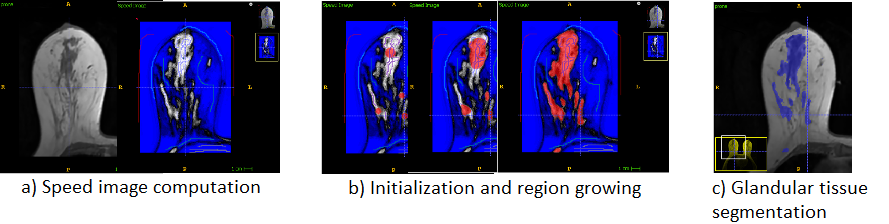
\includegraphics[width=\textwidth,height=\textheight,keepaspectratio]{figures/segmentation.png} }
\caption{Example of tissues segmentation: glandular tissue.}
\label{segmentation}
\end{figure}
\end{center}

The segmentation process for one tissue type takes place in 3 steps (see fig \ref{segmentation}): 
\begin{enumerate}
\item Computation of a new synthetic image representing the probability of a pixel to belong (value 1) or not (value -1) to a given tissue type. The probability is computed using random forest algorithm. The training data is given by the user and include state and space characteristics as: voxel grey intensity, voxel's neighbors intensity (neighborhood radius equal to 4) , $(x,y,z)$ voxel position. \\

\item Initialization: One or more seeds point are placed in the synthetic image in the regions corresponding to our region of interest. These points will be grown accordingly to the computed probability to form the segmented structure in the next step. \\
\item Region growing: evolution of the placed seeds. The placed point will evolve on time according to the synthetic images: boundary expending on the positive regions, boundary contracting over the negatives ones.\\
\end{enumerate}
\subsection{Subject-specific Finite Element mesh generation}
Subject specific Finite Element (FE) mesh is generated using Bolt software \cite{bolt}.

\begin{center}			  
\begin{figure}[h]
\centerline{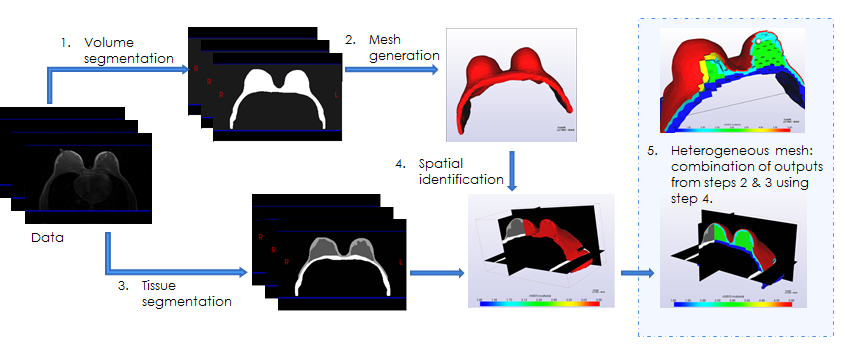
\includegraphics[width=\textwidth,height=\textheight,keepaspectratio]{figures/FEMesh.png} }
\caption{Subject-specific heterogeneous mesh generation.}
\label{femesh}
\end{figure}
\end{center}

 First a homogeneous hexa-dominant mesh is generated from the volumes (breast + muscle). Next, for each finite element a material type is assigned by spatial identification with the segmented data. The tissue type assigned to an element is the tissue with a maximal number of pixels inside the element's convex envelope. At this step the finite element mesh is composed of 3 type of materials: pectoral muscle, adipose tissue, glandular tissue. Finally, two hexahedral layers are added at the external surface of the breast mesh: one of 0.1 mm and the second one of 2 mm (see fig. \ref{femesh}). These layers will represent the fascia and the skin layer respectively.



\subsection{Biomechanical soft tissues model}
 The large deformation of breast tissues was modelled using finite strain formulation of the finite element method from the ANSYS commercial package. In our model we will consider 5 types of tissues: pectoral muscle, adipose tissue, glandular tissue, superficial fascia and skin. In reality, the breast tissues are: anisotropic because of the Cooper’s ligament reinforcing the breast in the muscle-to-skin direction; quasi-incompressible due to the presence of lactiferous ducts and blood vessels; heterogeneous and hyperelastic. Here, the breast soft tissues will be modelled as homogeneous, isotropic, quasi-incompressible and hyperelastic models.  To model the mechanical response of breast tissue we are using a Neo-Hookean material with the strain-energy potential:
$$W=\frac{\mu}{2}(I_1 -3) + \frac{k}{2}(J-1)^2$$
Here $\mu$ is the initial shear modulus, $k$ is the Bulk modulus, $I_1$ the first invariant of Cauchy stress tensor and $J$ the volume ratio. The material parameters $\mu$ and $k$ can be related to the Young's modulus $E$ and Poisson ratio $\upsilon$ through the relations: 
$$\mu = \frac{E}{2(1+\upsilon)}  \ \   k=\frac{E}{3(1-2\upsilon)}$$ 

The Young's modulus and Poisson ratio are defined for each material separately.
\subsection{Boundary conditions}
The bibliography presents two type of boundary conditions (see appendix \ref{mechanical_models_table}): zero-displacement nodes defined on the surface between the breast and the pectoral muscle and sliding surfaces between the breast and pectoral muscle. As we include the pectoral muscle in the model, we use zero-displacement conditions for the nodes of its posterior surface. The muscle and breast tissues are perfectly sticked together by sharing the same nodes on the intersection surface. The skin and fascia layers are extending up to the pectoral muscle in order to limit the soft tissues deformation in the region of axilla ends, shoulder and inferior part of the rib cage. 
\subsection{Estimating the stress-free breast configuration}

As mentioned before, the estimation of the stress-free breast configuration is important for breast biomechanical modeling. For the methods based on patient specific data the finite element mesh is computed using images acquired with breast tissues thar are pre-stressed because of gravity loadings. As the internal pre-stress of the tissue is impossible to measure, estimation methods are used. The main approach to this problem is to estimate the unloaded geometry (the reference state) which is considered to be stress-free, then to simulate the breast deformation due to the gravity in order to estimate the pre-stress conditions.   The method used to compute the "stress-free" geometry is based on the one proposed by \cite{ carter_biomechanical_2009} and adapted later by \cite{eiben_breast_2014} and \cite{eder_comparison_2014}. 
\begin{center}			  
\begin{figure}[h]
\centerline{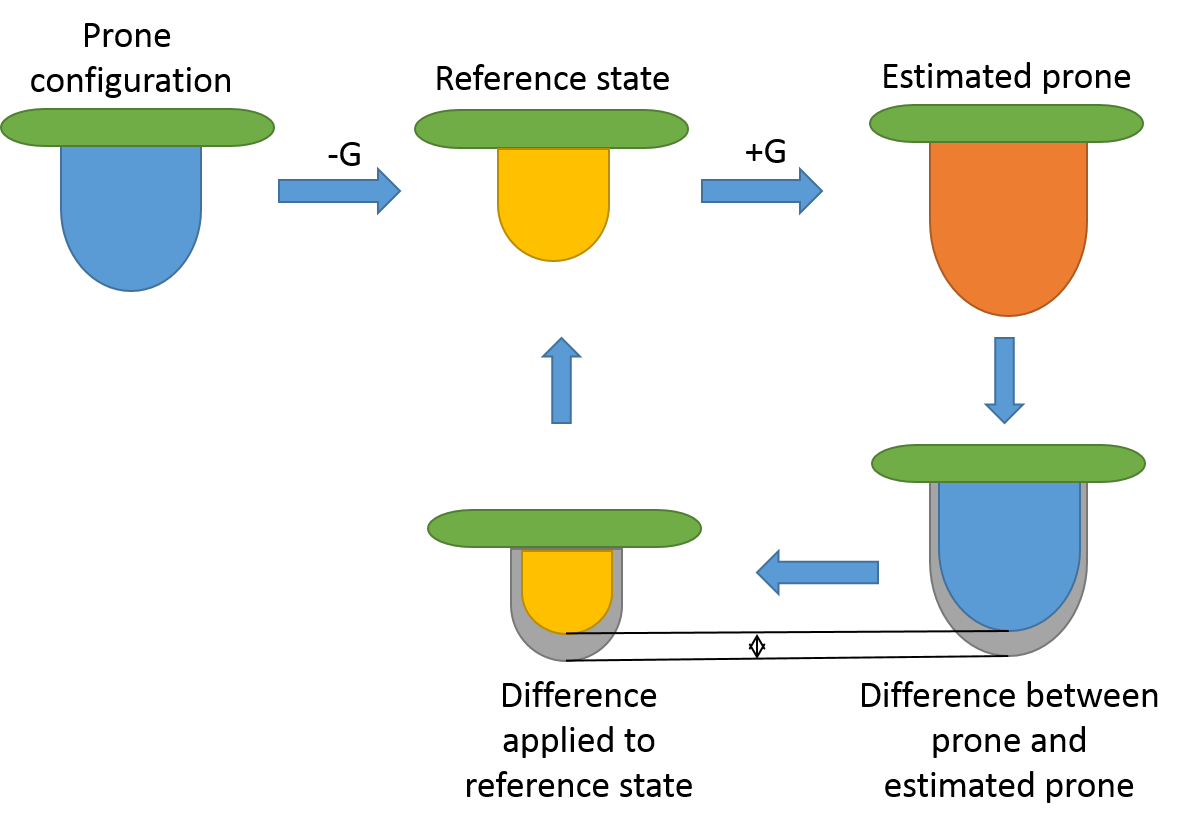
\includegraphics[width=\textwidth,height=\textheight,keepaspectratio]{figures/IFP.png} }
\caption{Prediction-correction iterative algorithm for stress-free geometry estimation.}
\label{IFP}
\end{figure}
\end{center}

The original method uses the prediction-correction iterative scheme represented in fig. \ref{IFP}. The process begins by considering that the initial geometry generated from MR images (fig.\ref{IFP} a) prone configuration) has zero internal stress. Then, the gravity is applied in the reverse direction which gives a first estimation of initial stress-free state (fig.\ref{IFP} b) reference state).
Next, the gravity is reloaded in the natural direction and the guess of the deformed state is given (fig. \ref{IFP} c) estimated prone). At this step the difference  between the estimated deformed geometry and the measured one (fig. \ref{IFP} d)) is computed. The difference between the two surfaces is applied as a nodal displacement on the reference state (fig.\ref{IFP} e)). The process is repeated until the convergence is achieved.

Here, the same iterative process is used but with a more adapted update of the reference state.


%\begin{center}			  
%\begin{figure}[h]
%\centerline{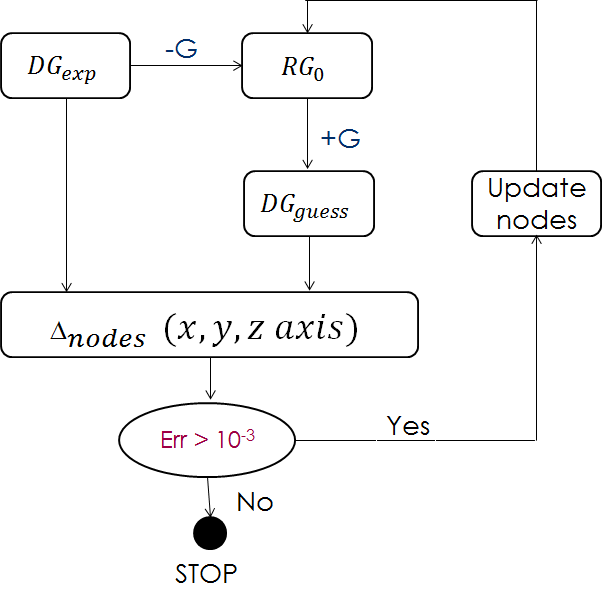
\includegraphics[scale=0.7]{figures/iterativeAlgorithm.png} }
%\caption{Prediction-correction iterative scheme for stress-free geometry estimation.}
%\label{itAlgo}
%\end{figure}
%\end{center}


\subsubsection*{First guess of stress-free geometry}
The first estimation of the stress-free geometry is very important for the method accuracy and convergence. Generally, the iterative optimization methods are dependent on their initialization. If initialization is not situated in the solution's neighborhood the optimization can be stuck in a local extrema or have problems to achieve the convergence. As we dispose of two opposite breast deformed geometries (supine and prone position) we combined them in order to compute an "intermediary geometry" which will be used as initialization of the optimization process. The combination of the two geometries is purely geometrical and has no biomechanical meaning.

The combination of the two geometries is performed in 2 steps: first, a mesh morphing method is applied to match the supine geometry to the prone geometry. The morphing algorithm used here has been developed by \cite{bucki_fast_2010} and estimates an elastic transformation from a source mesh to a target mesh preserving the elements regularity. The transformation is computed using the surface nodes only but is valid for the entire deformation space. A regularization factor limits excessive space distortions. In this context one can translate the finite element mesh from supine configuration to the prone one with limited element distortions.

Once this mesh morphing is completed the two configurations are represented by the same FE mesh, i.e. the same number of nodes and the same number of elements. Therefore, we are able to compute the geometrical mean between node's locations. Finally, our initialization geometry is computed by the FE mesh having each node at the mean location between the prone and supine configuration. 
 
\subsubsection*{Update computation}

In the previous versions of the iterative algorithm, the update calculation for the initial state is computed for each node of the finite element mesh. The finite element mesh used in our simulations is composed by elements of mean edge length of $4mm$. An excessively large number of nodes mean too many conditions for the optimization problem. Thus, the geometry optimization is hyper-constrained and the convergence is achieved too fast without finding the solution. To avoid this problem, we propose an adapted update of the reference geometry. In this scope, instead using all mesh nodes for the update estimation, we will compute an elastic transformation to map the surface nodes from estimated data to the measured one.

As proposed by \cite{ carter_biomechanical_2009}, from the estimated stress-free configuration the deformed geometry is computed by applying the gravitational forces in their natural direction: forward to simulate the prone position or backward to simulate the supine position. Then, using the mesh registration algorithm, an elastic transformation is computed to map the surface nodes of estimated deformed geometry to the surface generated from MRI. Then, the computed node displacement is applied on the stress-free geometry. The process is repeated until the convergence is achieved.


\section{Results and Discussions}
\subsection{Breast soft tissue elastic parameters.}
The values of the soft tissues presented in the literature range from 0.1 kPa to 57kPa. The purpose of this experiment is to investigate the model sensibility to the tissue elasticity and to find a smaller interval for the elastic modulus. In order to evaluate the impact of tissues elasticity on the breast mechanics we have made several basic simulations. For the first test we assumed that the skin, the glandular and adipose tissues are described by the same Neo-Hookean law. The Poisson Ratio of the pectoral muscle and the breast soft tissues was fixed at 0.45. The elastic modulus of the pectoral muscle was fixed at $30 kPa$ and the breast modulus was set to $0.5kPa$, $1kPa$, $5kPa$, $10kPa$ et $20kPa$ consecutively.

The simulation process is divided in 2 steps. First, we consider the supine configuration with zero-internal forces and then we apply the reverse gravity. The new estimation is supposed to by the "stress-free" breast configuration.  Next, the gravity is applied in the forward direction in order to estimate the prone breast configuration. From the estimated prone breast geometry, the 3D location of the nipple is registered and compared to the nipple position in the experimental prone position. Table \ref{nippleError} shows the Euclidean distance between nipple location in the estimated geometry and the one in measured in the MR images geometry. We observe that an elastic modulus of $20 kPa$ for breast is too stiff, the maximal node displacement is equal to $2.23 mm$ which is far too small to describe the breast mechanics from supine to prone configuration.  
\begin{table}[h]
\begin{center}
\begin{small}
\begin{tabularx}{15cm}{|p{2cm}|X|X|X|X|X|X|}
\hline
Side & D (mm) E=0.5kPa &D (mm) E=1kPa &D (mm) E=5kPa&D (mm) E=10kPa&D (mm) E=20kPa & supine\\
\hline
\rowcolor{mygray}Left &17.00&29.32&37.17&38.05&38.80& 39.11\\
Right &6.62&25.94&37.43&38.72&39.88&39.89\\
\rowcolor{mygray}Max Disp. &23.30&9.12&3.21&2.66&2.23&\\
\hline


\end{tabularx}
\end{small}
\caption{Nipple location error computed between estimated and experimental loaded prone breast position. D= euclidean distance from estimated location to experimental location. Max Disp = maximal nodal displacement for corresponding elastic modulus. Supine = euclidean distance of nipple location between supine and prone position}
\label{nippleError}
\end{center}
\end{table}

\begin{center}			  
\begin{figure}[H]
\centerline{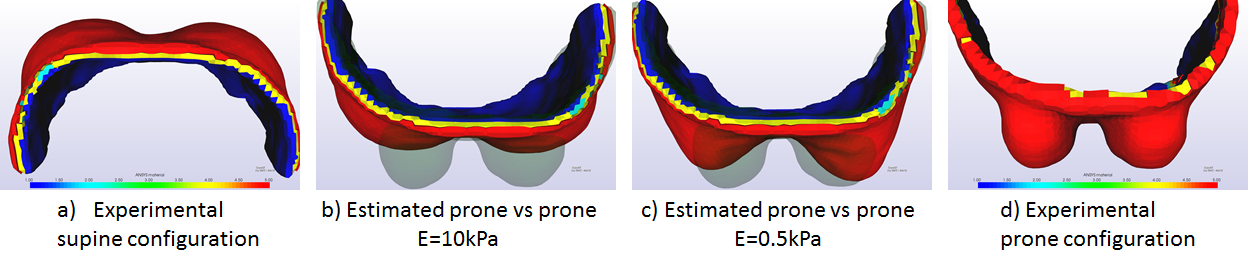
\includegraphics[scale=0.7]{figures/elasticModulus.png} }
\caption{Breast deformation depending on elastic modulus.}
\label{elasticModulus}
\end{figure}
\end{center}


According to the obtained results, we can conclude that the elastic modulus of breast soft tissues is more likely to by around 1 kPa. Most of the values given in the literature underestimate the breast deformation (see fig. \ref{elasticModulus}). Same results have been obtained by \cite{carter_determining_2009, han_development_2012, Rajagopal_creating_2008} using a similar FE method and experimental measurments. However, their results do not describe the intra-subject elasticity variation. We have seen that the elastic properties for one subject can change for about 30\% within a month (\cite{lorenzen_menstrual-cycle_2003}); our results show that the biomechanical breast model is very sensitive to the tissues elastic modulus; therefore, it is very important to have a good approximation of the elastic parameters. 

Our model included only adipose tissues; it must be mentioned that the glandular tissue and human skin are stiffer than the adipose tissue. Thus, we must consider that adding this tissues in the model will rigidify the entire structure.

An optimization method of elastic parameters such as the one presented by \cite{carter_determining_2009} must be developed in order to estimate them for each subject and for each type of tissue.

\subsection{Skin impact in breast mechanics.}

The skin is covering the breast tissues like an elastic envelope. As skin is stiffer than the breast soft tissues, its mechanical properties govern the global breast mechanics. In this section we discuss the influence of the skin layer on breast mechanics deformed by gravity loading. 

In this scope, we have done simulation using 2 breast models. The first one is computed from 3 type of materials: muscles, breast soft tissues (glandular + adipose) and skin. The second one contains only muscle and breast tissues. All tissues are quasi-incompressible Neo-Hookean materials. According to the literature and to our previous results we chose the elastic parameters for skin, breast and muscle equal to $10 kPa$, $1 kPa$ and $30kPa$ respectively. For this section we consider the prone configuration as the "stress-free" one (i.e zero internal stress) and we simulate the up-right breast configuration with and without the skin layer. 

\begin{center}			  
\begin{figure}[h]
\centerline{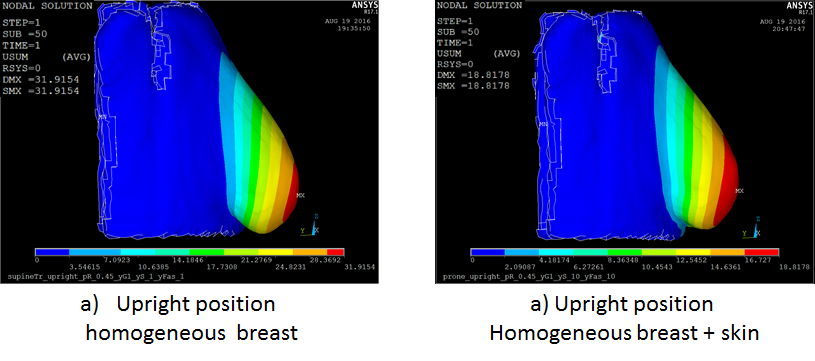
\includegraphics[scale=0.7]{figures/upright-position.png} }
\caption{Upright breast configuration with and without skin layer.}
\label{upright}
\end{figure}
\end{center}

Figure \ref{upright} shows the difference between the upright position computed with and without skin layer. The skin layer can reduce the breast nodal displacement up to 30\%. 

\subsection{Stress-free configuration estimation.}
The estimation of the stress-free configuration is a big challenge in breast biomechanical modeling. As we assume that the breast tissues are non-linear material, a simple reverse gravity method is not relevant. Thus we implemented the iterative scheme from \cite{carter_determining_2009} in order to estimate the reference geometry (see fig. \ref{iterativeRG}, left column). The model contains 3 types of tissues as hyperelastic model with elastic modulus equal to $10kPa$, $1kPa$ and $30kPa$ for skin, breast and muscle respectively.  

\begin{center}			  
\begin{figure}[h]
\centerline{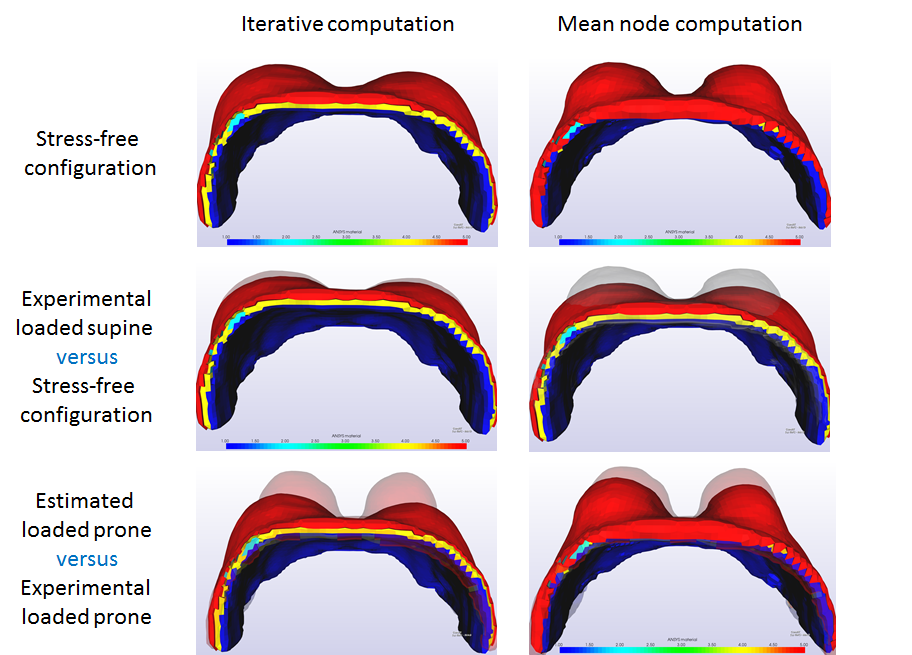
\includegraphics[scale=0.8]{figures/iterativeVsMean.png} }
\caption{Zero-stress geometry estimation results.  }
\label{iterativeRG}
\end{figure}
\end{center}


As we can see in fig.\ref{iterativeRG} (second line) the estimated stress-free configuration is too close to the experimental supine configuration. The reason of the poor approximation is the assumption of zero internal stress in supine position at first iteration and also non adapted elastic parameters. Firstly, the chosen elastic materials turn the breast in a too stiff structure, therefore the large deformations are not achieved. Secondly, the optimization algorithm is initialized with the supine geometry with the assumption of zero internal stress, the breast geometry being too far from the reference one, the algorithm can be stopped in a local minimum.   

Applying on method "mean node computation", fig.\ref{iterativeRG} thus introducing the new stress-free geometry (fig \ref{iterativeRG} first line, second column) which represents only the first approximation of the stress-free configuration, i.e. without applying any iterative algorithm, the results are improved. The estimated breast geometry in prone position is closer to the experimental data. The difference between the 2 geometries can be improved by optimizing the materials elastic parameters. By taking the elastic modulus for breast and skin equals to $0.3 kPa$ and $10kPa$ (\cite{carter_determining_2009}) the estimated supine and prone configuration are considerably improved. Fig \ref{optimizedParam} shows the obtained results for loaded breast geometry in supine and prone positions compared to the measured geometries in supine and prone positions.  

\begin{center}			  
\begin{figure}[h]
\centerline{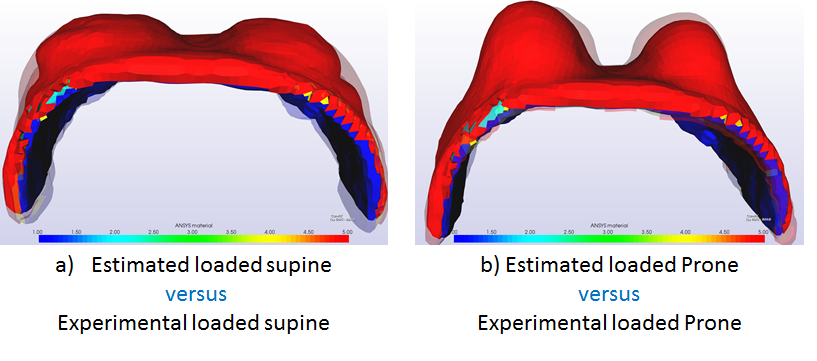
\includegraphics[scale=0.8]{figures/estimated_PS_Mesn_3e-1.png} }
\caption{Estimated prone and supine configurations versus experimental measures. Elastic parameters: muscle= 30kPa, breast=0.3 kPa, skin= 10kPa }
\label{optimizedParam}
\end{figure}
\end{center}
\section{Conclusion and Perspective}
Modeling breast deformations is a challenging problem due to its anatomical complexity. First of all, breast heterogeneity must be included in the model. Contrary to others works, our model considers 3 type of tissues: the muscle, the breast and the skin. The results show a huge sensibility of the model to the tissue elastic parameters. For examples the breast deformation can by reduced by about $30\%$ if the skin layer is modeled. Therefore, in the future we plan to include in our model more tissues types as glandular and adipose tissue.

 As the breast tissues are extremely soft and the elastic parameters variate depending not only on the subject but also on their physical and physiological conditions, the values given in the literature cannot be generalized to our volunteers. Therefore, the estimation of individual elastic parameters is necessary. At the first step of this work, the elastic parameters of breast tissues are estimated by a manual exhaustive research between the minimal and maximal values found in the literature. The best fitting of the simulated results to the measured data was obtained with an elastic modulus of 30kPa for muscle, 0.3 kPa for breast and 10 kPa for skin. The obtained values are very small compared to ones given by the literature: 20 kPa for Breast tissues and 80 kPa for skin. Such a large difference can be explained by the various conditions during data acquisition and different mathematical models. The large variation of the elastic modulus motivates us to implement an automated optimization algorithm which will estimate the individual elastic parameters for each subject.      
 
Another important difficulty in breast mechanics modeling is the unknown "stress-free" configuration, which in in-vivo conditions, cause to the gravity, is not easy to obtain with experimental measurements. We have implemented a well-known method based on the iterative fixed point algorithm in order to estimate the "stress-free" geometry. The obtained results shown an unsatisfactory accuracy (see fig. \ref{iterativeRG}). In order to improve this, we have proposed a different estimation of the "stress-free" geometry. Based on a combination between the geometries in prone and supine positions. This assumption improves the obtained results but still need more corrections. Therefore, we intend to integrate the two methods by using the combined geometry as an initialization for the iterative algorithm.  

 On the other hand, the deformations that are usually applied to breast tissues, either gravity loading or paddle compression, are considerable. Thus, excessive elements distortions and respectively inaccurate results and numerical instability are often observed. It is difficult to emphasize an optimization algorithm on poor quality FE mesh, since in this situations, numerical problems stop the iterative process before the convergence is achieved. A possible overcome is to implement a regional re-meshing process during the solution computation. At each computation step, the mesh quality will be supervised: if an element overtakes the fixed quality threshold, the element and its neighborhood is re-meshed.  
 
To sum up, we plan to compute the patient specific elastic parameters by implementing an optimization algorithm. The method estimate the elastic parameters with the best match between supine and prone positions. Concerning the stress-free configuration, we intend to improve the fixed point algorithm by giving a new geometry initialization. The new method will compute the geometry updates based on the surface nodes only. The iterative method will give a unique "stress-free" geometry given the tissue elastic parameters, the prone and the supine breast configurations. The difficulties that we found in implementation of both methods is the poor elements quality of the finite element mesh. Even if we start with a high- quality mesh, after one iteration the elements are distorted and no further iterations are possible. In order to solve this problem, we plan to include in the simulation workflow a re-meshing step in order to control the elements quality in case of large deformations.  




	

